\documentclass[10pt, unicode]{beamer}
\usepackage[english]{babel}
\usepackage[utf8x]{inputenc}
\usepackage[T1]{fontenc}
\usepackage{bbding}
\usepackage{animate}
\usepackage{xcolor}
\usepackage{color}
\usepackage{colortbl}


\usepackage{numprint}
\npthousandsep{\,}
\newcommand{\quotes}[1]{``#1''}
\usetheme{Berlin}
\usecolortheme{beaver}

%title page
\title{Optimization and Applications of Deep Learning algorithms for Super Resolution in MRI}
\author{Mattia Ceccarelli}
\institute{Master Degree in Physics \\ Alma Mater Studiorum - University of Bologna}
\date{A.Y. 2019-2020}

\begin{document}

\begin{frame}
 \maketitle
 
  {\bf Supervisor}:  Prof. Gastone Castellani
 
  {\bf Co-Supervisor}: Dott. Nico Curti

\end{frame}

\begin{frame}{Introduction}
 
\end{frame}


\begin{frame}{Single Image Super Resolution}{What is Super Resolution?}

  \setbeamercolor{block title example}{fg=black, bg=green!40!white}
  \setbeamercolor{block body example}{fg=black, bg=green!20!white}
  
  \scriptsize{Two main groups of techniques : }
  \begin{itemize}
   \item SR microscopy, which aim is to overcome the diffraction limits with a complex laboratory setup.
   \item SR algorithm, which aim is to enhance the spatial resolution of an image for different purpose such as object detection, segmentation and improve its visual quality
  \end{itemize}

  \setbeamertemplate{itemize items}[ball]

  \begin{exampleblock}{Super resolution procedure}
    \begin{itemize}

      \item Start from a prior-known High Resolution (HR) image;
      \item Rescale the image obtaining its Low Resolution (LR) counterpart;
      \item Feed a super-resolution model with the LR image trying to obtain as output its HR version;
      \item With the trained model we can re-apply the up-sampling procedure and further increase the HR quality*.

    \end{itemize}
  \end{exampleblock}

  \vspace{0.5cm}
  \scriptsize{* This is even more efficient if we think about a \textbf{zoom} procedure.}

\end{frame}

\begin{frame}{Deep Learning model}

  \begin{itemize}
    \item Neural Networks are mathematical models commonly used in data analysis.
    \item From a theoretical point-of-view we can define a Neural Network as \textbf{a series of non-linear multi-parametric functions}.
    \item Neural Networks are considered as \textbf{Universal Function Approximators}.
  \end{itemize}

  \begin{figure}[hbp]
    \centering
    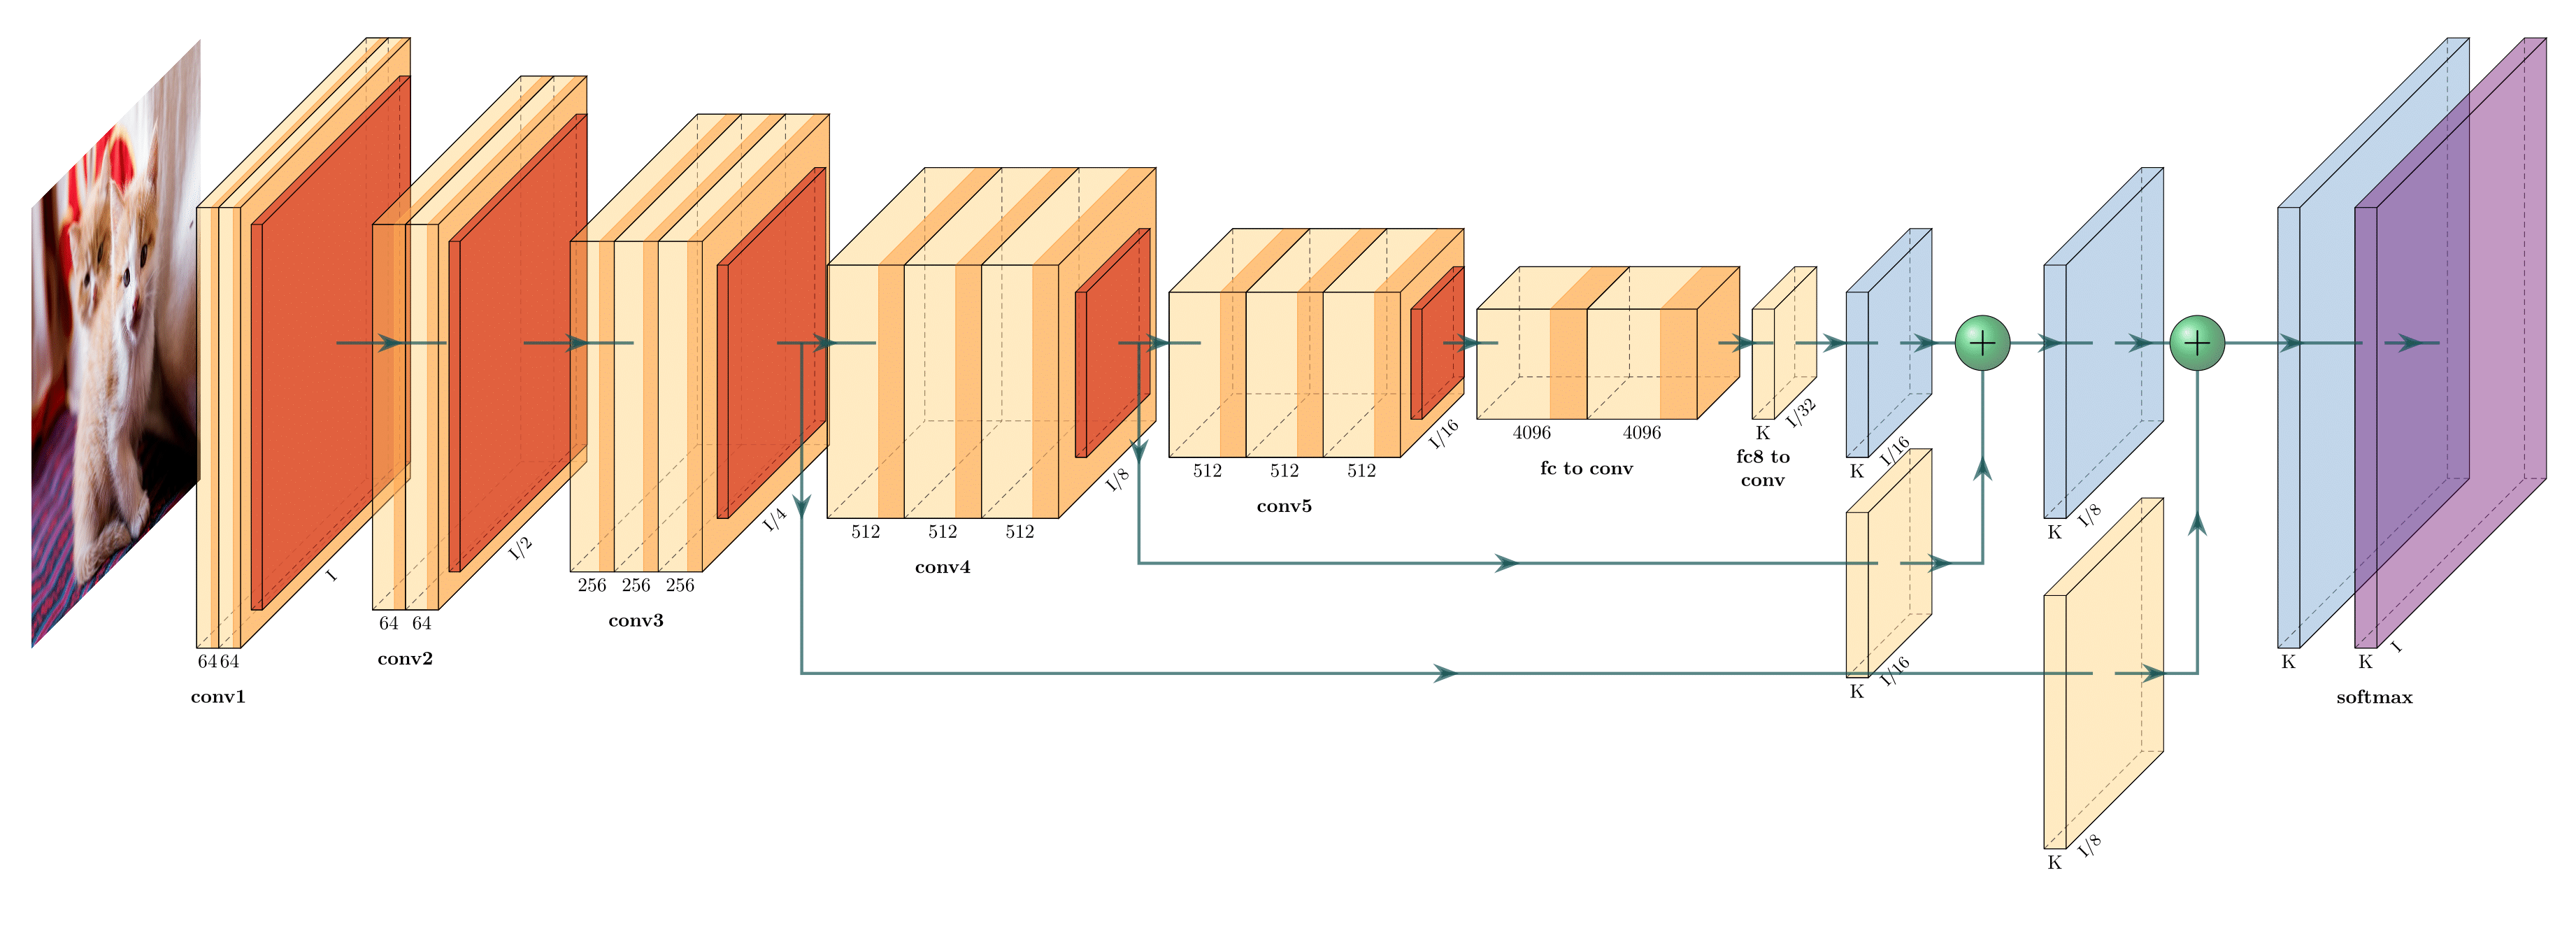
\includegraphics[width=0.85\textwidth, height=0.29\textwidth]{images/net_scheme.png}
    \caption{\scriptsize{Neural Network model scheme.
             The model is composed by a series of layers made by interconnected computational units.
             The connections between layers can be serials or parallels and each layer models a pre-determined mathematical function.
            }}
  \end{figure}

\end{frame}

\begin{frame}{Deep Learning}{Neural Network models}
  
  \begin{itemize}
    \item The supervised training of neural network happens by feeding the model 
          with labeled example, that are couples of inputs and expected outputs.
    \item Then, the output is compared with the label by means of a \textbf{cost function}, which is a measure of the error made by the network.
          
          The objective is to modify the \textbf{parameters} of the model to minimize the cost function.
    
    \item {Commonly, we think about Neural Network models as tools to \textbf{reduce} problems dimensionality, i.e. starting from high-dimensional data (e.g $w\times h\times c$ image) the model predicts a class (single number)}.

    \item {In Super Resolution we have no classes but the desired output is also an image.
          Single Image Super Resolution tasks start from an image and the aim is to reconstruct its HR counterpart.}
  \end{itemize}
  
  \setbeamertemplate{itemize items}[ball]

  %\begin{block}{Objectives}
   % \begin{itemize}

    %  \item Optimization and extension of state-of-art Neural Network libraries;

     % \item  Development of two novel libraries, for education and analytic purposes, respectively;

      %\item Improve parallelization strategies to reach the best computational performances in cluster machine without GPUs supports;

   % \end{itemize}

  %\end{block}

  %\begin{alertblock}{}
   % All the algorithm and codes developed are \textbf{tested}, \textbf{documented} and \textbf{public available}!

    %\quad

    %\textbf{Reference:} \url{https://nico-curti2.gitbook.io/phd-thesis} (GitBook documentation).
  %\end{alertblock}

\end{frame}
 

% \begin{frame}{State-of-art libraries}{Why another library?}
% 
%  % \scriptsize{A wide range of documentations and implementations have been written on Deep Learning and it is more and more hard to move around the different sources.}
% 
%   \scriptsize{Leaders on this topic are the multiple open-source Python libraries available on-line as \href{http://tensorflow.org}{Tensorflow}, \href{http://pytorch.org}{Pytorch} and \href{http://doi.acm.org/10.1145/2647868.2654889}{Caffe}.}
% 
%   \begin{columns}
% 
%     \begin{column}{0.5\textwidth}
% 
%       \begin{block}{Pros}
%         \begin{itemize}
%           \item[$\diamond$] Simplicity in writing complex models in a minimum number of code lines;
%           \item[$\diamond$] Simplicity of the \textsf{Python} language;
%           \item[$\diamond$] Extremely efficient in GPU environments;
%         \end{itemize}
%       \end{block}
%     \end{column}
%     \begin{column}{0.5\textwidth}
% 
%       \begin{alertblock}{Cons}
%         \begin{itemize}
%           \item[$\diamond$] Steep learning curve for complex applications or algorithm modifications;
%           \item[$\diamond$] They are not designed for CPU performances;
%         \end{itemize}
%       \end{alertblock}
%     \end{column}
% 
%   \end{columns}
% 
%   \vspace{0.5cm}
% 
%   \scriptsize{Only a small part of the research community uses deeper implementation in \textsf{C++} or other low-level programming languages.}
%   \scriptsize{About them it should be mentioned the \textsf{darknet project} of Redmon J. et al. which created a sort of standard in object detection applications using a pure \textsf{Ansi-C} library.}
% 
% \end{frame}

\begin{frame}{Frameworks}{Byron and NumPyNet}
 \scriptsize
  \setbeamercolor{block title alerted}{fg=black, bg=orange!40!white}
  \setbeamercolor{block body alerted}{fg=black, bg=orange!20!white}

  \setbeamertemplate{itemize/enumerate body begin}{}
  \setbeamertemplate{itemize/enumerate subbody begin}{}

  \begin{alertblock}{Byron \hfill
\includegraphics[width=0.02\textwidth]{images/cpp.png}}
    \begin{itemize}
      \item The library is written in \textbf{pure \textsf{C++}} with the support of the modern standard 17.

      \item The library is \textbf{optimized for image processing} (probably the most common task in biomedical research).

      \item Starting from the \textsf{darknet project} backbone, \textsf{Byron} introduces \textbf{numerous improvements and fixes}.

      \item The library is also \textbf{completely wrapped} using \textsf{Cython} to enlarge the range of users also to the \textsf{Python} ones.
    
    \end{itemize}
  \end{alertblock}
  
  \setbeamercolor{block title alerted}{fg=black, bg=blue!40!white}
  \setbeamercolor{block body alerted}{fg=black, bg=blue!20!white}

  \setbeamertemplate{itemize/enumerate body begin}{}
  \setbeamertemplate{itemize/enumerate subbody begin}{}

    \begin{alertblock}{NumPyNet}
    \begin{itemize}
      \item The library is written in \textbf{pure \textsf{Python}} and the only external library is Numpy (a common package for scientific research). 

      \item A minimal mathematical documentation associated to each script and a wide range of comments inside the code.

      \item NumPyNet tries to overcome the common ``black-box'' idea of Neural Network using simple and readable Python code.
      
      \item useful to test optimized code

    \end{itemize}
  \end{alertblock}

  %\vfill\scriptsize{* The library was developed in collaboration with Dott. Baroncini.}

\end{frame}


% \begin{frame}{Standard up/down scaling algorithms}{Single Image Super Resolution}
% 
%   \setbeamertemplate{itemize items}[ball]
% 
%   \begin{columns}
%     \begin{column}{0.4\textwidth}
%       \scriptsize{Interpolation algorithms:}
%       \begin{itemize}
%         \item \textbf{Nearest};
%         \item \textbf{Bicubic};
%         \item \textbf{Lanczos};
%       \end{itemize}
% 
%       \scriptsize{The best compromise between computation cost and efficiency is given by the Bicubic interpolation algorithm}.
%       \scriptsize{Given a pixel, the interpolation function evaluates the 4 pixels around it applying a filter given by the equation:}
%     \end{column}
%     \begin{column}{0.6\textwidth}
%       \begin{figure}
%         \centering
%         \def\svgwidth{\textwidth}
%         \input{./up_down_sampling.pdf_tex}
%         %\caption{\tiny{Up/Down sampling with scale factor equal to 2.}}
%       \end{figure}
%     \end{column}
%   \end{columns}

%   \
%   \begin{equation*}
%   \hspace{-0.75cm}\scriptsize{
%   k(x) = \frac{1}{6} \left\{ \begin{array}{rc}
%     (12 - 9B - 6C) |x|^3 + (-18 + 12B + 6C) |x|^2 + (6 - 2B)           & \mbox{if}        |x| < 1 \\
%     (−B − 6C) |x|^3 + (6B + 30C) |x|^2 + (−12B − 48C) |x| + (8B + 24C) & \mbox{if} 1 \leq |x| < 2 \\
%     0                                                                  & \mbox{otherwise}         \\
%     \end{array}
%     \right.
%   }
%   \end{equation*}
%   \\
%   \scriptsize{where $x$ identifies each pixel below the filter.}
%   \scriptsize{Commonly values used for the filter parameters are $B=0$ and $C=0.75$ (used by \textsf{OpenCV} library) or $B=0$ and $C=0.5$ used by \textsf{Matlab}}.
% 
%   \scriptsize{\textbf{NOTE:} the nearest interpolation could be achieved also using \emph{Pooling} algorithm.}

% \end{frame}

\begin{frame}{Image Quality}{Single Image Super Resolution}

  \setbeamercolor{block title}{fg=black, bg=blue!40!white}
  \setbeamercolor{block body}{fg=black, bg=blue!20!white}

  \setbeamercolor{block title alerted}{fg=black, bg=orange!40!white}
  \setbeamercolor{block body alerted}{fg=black, bg=orange!20!white}

  \setbeamertemplate{itemize/enumerate body begin}{\scriptsize}
  \setbeamertemplate{itemize/enumerate subbody begin}{\scriptsize}

  \scriptsize{The most common image quality evaluator is given by our eyes.}

  \scriptsize{Quantitative evaluations:}

  \begin{columns}
    \begin{column}{0.4\textwidth}
      \hspace{-0.75cm}
      \begin{block}{PSNR - Peak Signal to Noise Ratio}
        \begin{itemize}
          \item It establishes the compression lossless of an image;

          \item Equation:

          \begin{equation*}
          \hspace{-0.75cm}
          PSNR = 20 \cdot \log_{10}\left( \frac{\max(I)}{\sqrt(MSE)} \right)
          \end{equation*}
          \\
          where $\max(I)$ is the maximum value which can be taken by a pixel in the image and $MSE$ is the Mean Square Error evaluated between the original and reconstructed images.
        \end{itemize}
      \end{block}
    \end{column}
    \begin{column}{0.65\textwidth}
      \begin{alertblock}{SSIM - Structural SIMilarity index}
        \begin{itemize}
          \item It evaluates the structural similarity between two images taking into account also the visible improvement seen by human eyes.

          \item Equation:

          \begin{equation*}
          \hspace{-0.75cm}
          SSIM(I, K) = \frac{1}{N}\sum_{i=1}^{N} \frac{(2\mu_x\mu_y + c_1)(2\sigma_{xy} + c_2)}{ ({\mu_x}^2 + {\mu_y}^2 + c_1)({\sigma_x}^2 + {\sigma_y}^2 + c_2) }
          \end{equation*}
          \\
          where $N$ is the number of arbitrary patches which divide the image and $c_1$ and $c_2$ parameters are fixed to avoid mathematical divergence.

        \end{itemize}
      \end{alertblock}

%       \begin{tabular}{lcc}
%         \hline \rowcolor{green!20!white}
%                           & \textbf{PSNR (dB)} & \textbf{SSIM ($\in [-1, 1]$)} \\
%         \hline
%         \textbf{Nearest}  & 25.118             & 0.847                         \\
%         \textbf{Bicubic}  & 27.254             & 0.894                         \\
%         \textbf{Lanczos}  & 26.566             & 0.871                         \\
%         \hline
%       \end{tabular}
    \end{column}

  \end{columns}

\end{frame}

\begin{frame}{EDSR - Enhanced Deep Super Resolution}{Super Resolution Models}
  \centering
  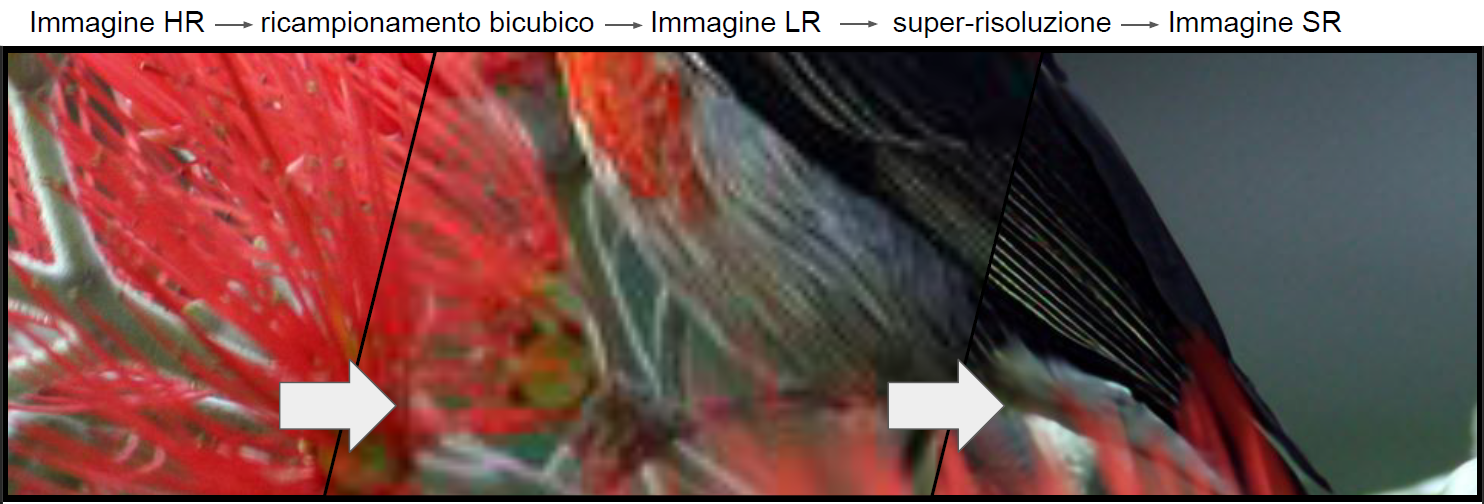
\includegraphics[width=0.78\linewidth]{images/compare.png}

  \setbeamercolor{block title alerted}{fg=black, bg=orange!40!white}
  \setbeamercolor{block body alerted}{fg=black, bg=orange!20!white}

  \begin{alertblock}{Architecture}
    \scriptsize{
    \begin{tabular}{lccc}
      \hline \rowcolor{orange!20!white}
                               &  Channels     & Filter     & Number of    \\
      \rowcolor{orange!20!white}
      Layer                    & input/output  & dimensions & Parameters   \\
      \hline
      Conv. input              & 3/256      & $3\times3$   & 6912          \\
      Conv. (32 residual block)   & 256/256    & $3\times3$   & 589824        \\
      Conv. (pre-shuffle)      & 256/256    & $3\times3$   & 589824        \\
      Conv. (upsample block)   & 256/1024   & $3\times3$   & 2359296       \\
      Conv. output             & 256/3      & $3\times3$   & 6912          \\
      \hline
    \end{tabular}
    }

    \vspace{0.5cm}
    \scriptsize{Average Time on $510\times339$ image: $576.92$~s.}

    \scriptsize{Winner of the \textbf{NTIRE 2017}. More than \textbf{40 million} of parameters}
  \end{alertblock}

\end{frame}

\begin{frame}{WDSR - Wide Deep Super Resolution}{Super Resolution Models}
  \centering
  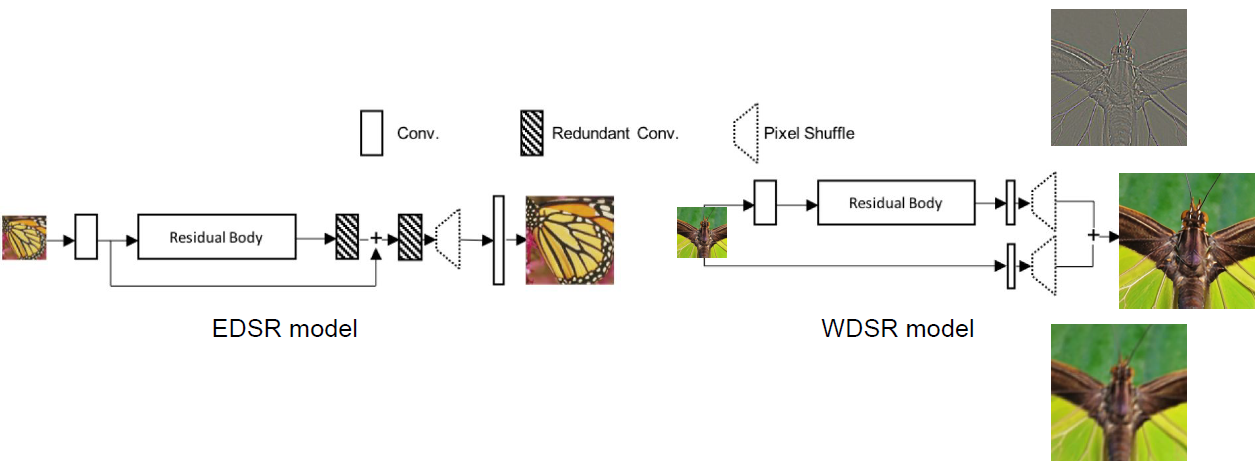
\includegraphics[width=0.7\linewidth]{images/SR_models.png}

  \setbeamercolor{block title}{fg=black, bg=blue!40!white}
  \setbeamercolor{block body}{fg=black, bg=blue!20!white}

  \begin{block}{Architecture}
    \scriptsize{
    \begin{tabular}{lccc}
      \hline \rowcolor{blue}
                                  &  Channels     & Filter     & Number of    \\
      \rowcolor{blue}
      Layer                       & input/output  & dimensions & Parameters   \\
      \hline
      Conv. input 1               & 3/32       & $3\times3$   & 864     \\
      Conv. 1 (32 residual block)    & 32/192     & $3\times3$   & 55296   \\
      Conv. 2 (32 residual block)    & 192/32     & $3\times3$   & 55296   \\
      Conv. (pre-shuffle)         & 32/48      & $3\times3$   & 13824   \\
      Conv. input 2 (pre-shuffle) & 3/48       & $5\times5$   & 3600    \\
      \hline
    \end{tabular}
    }

    \vspace{0.5cm}
    \scriptsize{Average Time on $510\times339$ image: $46.35$~s.}

    \scriptsize{Winner of the \textbf{NTIRE 2018}. $\sim3$ million of parameters, \textbf{less than $10\%$ of EDSR model}!}
  \end{block}

\end{frame}

\begin{frame}{Dataset}{downscaled MRI description}
 \begin{itemize}
  \item Dataset composed of 5 patients T1-weighted and T2-weighted with 176 slices 256 x 256
  \item Each sample has been donw-scaled with a bicubic algorithm with two different scale factors (x2 and x4)
  \item The LR images are then convoluted with a gaussian kernel with size 3, stride 1 and sigma 1
 \end{itemize}
 
 \begin{figure}
  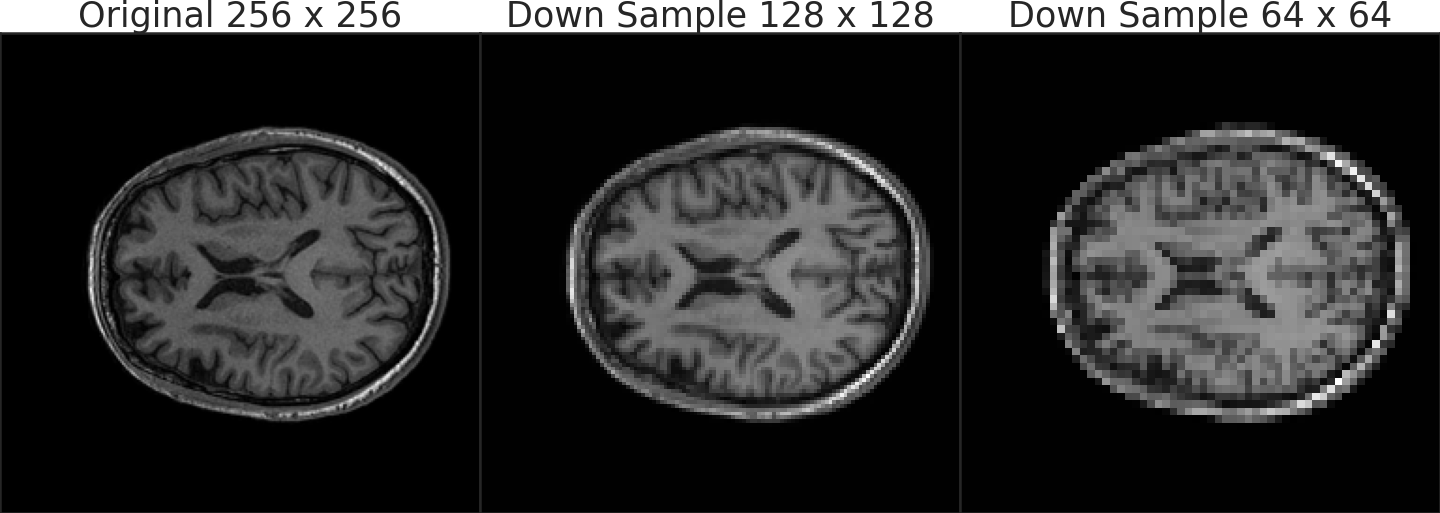
\includegraphics[scale=0.19]{./images/donwsamples}
 \end{figure}

\end{frame}


% Results.

\begin{frame}{Upsample Comparisons}{EDSR and Bicubic x2}

\begin{figure}
\centering
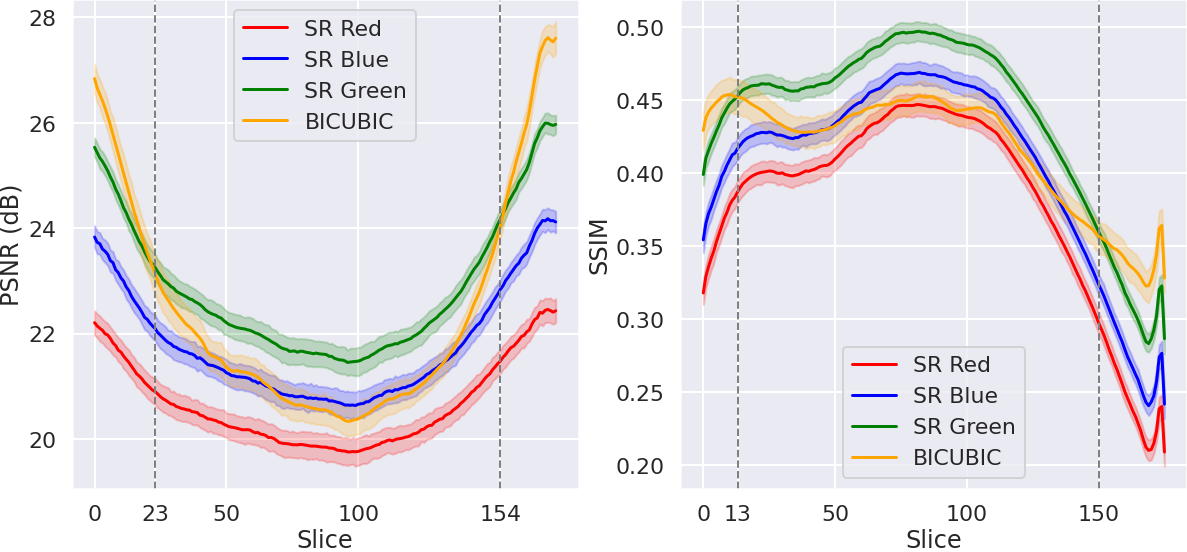
\includegraphics[scale=0.21]{./images/edsr_score_slide.png}
\caption{Average trends of PSNR (left) and SSIM (right) for the three channels (Red,
Blue, Green lines) of the Super Resolution EDSR model compared with the bicubic al-
gorithm scores (Yellow) as functions of the slices. The average is performed for every
patients and for every rotation. The dotted lines highlights the slices where the bicubic
and Super Resolution performances intersect.}
\end{figure}
\end{frame}

\begin{frame}{Upsample Comparisons}{WDSR and Bicubic x4}

\begin{figure}
\centering
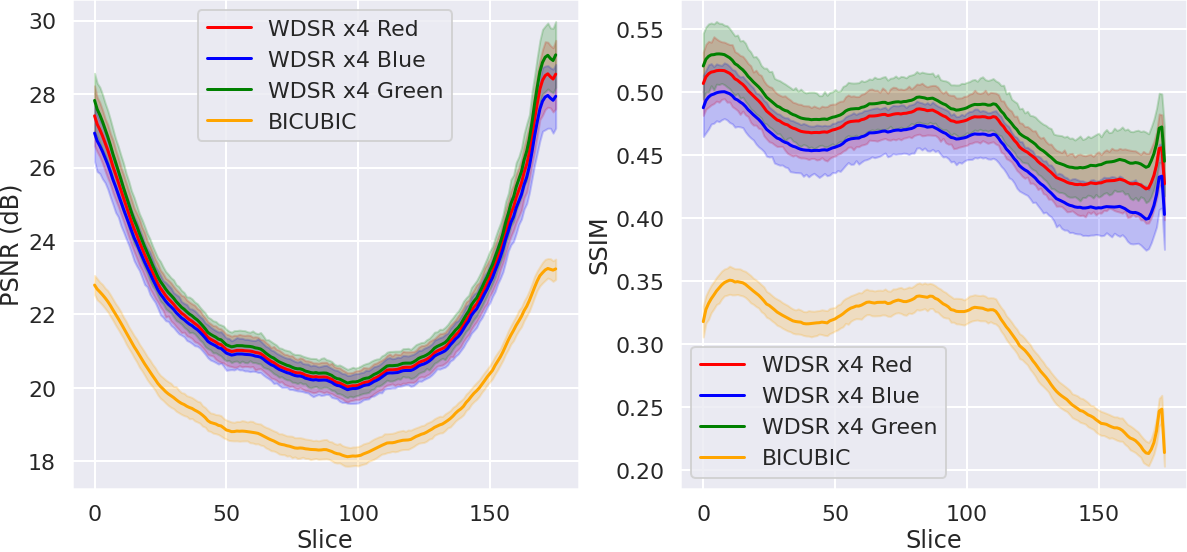
\includegraphics[scale=0.21]{./images/wdsr_score_slide.png}
\caption{Average trends of PSNR (left) and SSIM (right) for the three channels (Red,
Blue, Green lines) of the Super Resolution WDSR model compared with the bicubic algorithm scores (Yellow) as functions of the slices. The average is performed for every
patients and for every rotation.}
\end{figure}
 
\end{frame}

\begin{frame}{Upsample Comparisons}{WDSR and Bicubic x4}

\end{frame}

\begin{frame}{Scores by angle}
 
\end{frame}

\begin{frame}{Error Localization}{EDSR and Bicubic x2}

\begin{figure}
 \centering
 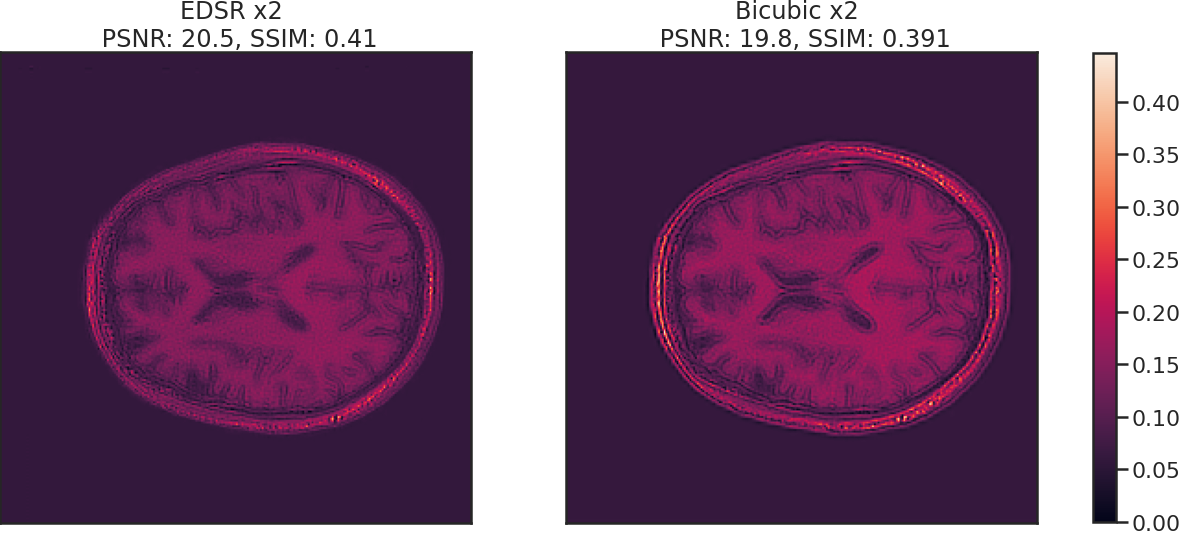
\includegraphics[scale=0.2]{./images/diff-edsr.png}
 \caption{Absolute differences of Super resolved image (left) and bicubic (right). in
both cases, the major differences seems to lies in the scalps of the subjecs. Though, it
can be seen that the background is not zero, which means it has an impact on the scores.}
\end{figure}
\end{frame}

\begin{frame}{Error Localization}{EDSR and Bicubic x2}

\begin{figure}
 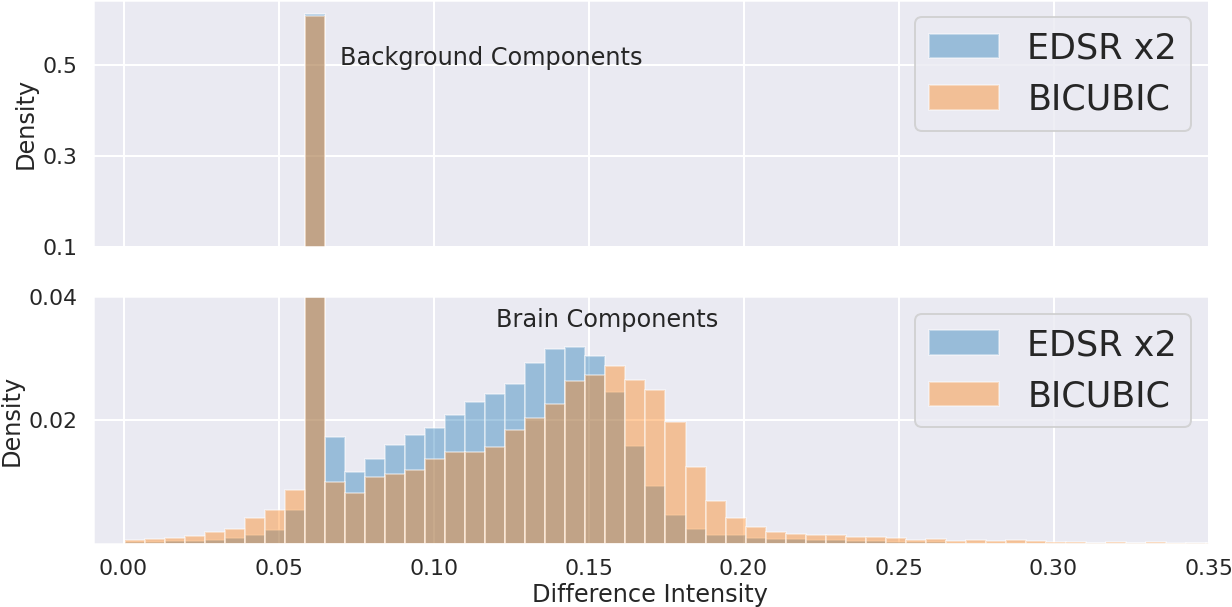
\includegraphics[scale=0.2]{./images/histo-edsr.png}
 \caption{Histograms of the distribution of absolute differences for the reconstruction
performed by EDSR (Blue) and by the bicubic algorithm (Orange). The histogram has
been cut between 0.04 and 0.1 on the y axis to better represent the lower parts.}
\end{figure}

 
\end{frame}

\begin{frame}{Brain Extraction}
 
\end{frame}


\begin{frame}{Conclusions}
\Large
  \begin{itemize}
   \item Two new libraries for Deep Learning applications wer proposed:
   \begin{itemize}
      \item {\bf NumPyNet} Focused on readability and educational purposes;
      \item {\bf Byron} a tool for efficient implementations in CPUs environment;
   \end{itemize}
   \item The results obtained using super-resolution are promising on applications on biomedical images
   \item DL models can generalize well, applying their ``knowledge'' to new datasets. 
  \end{itemize}

  
\end{frame}


\begin{frame}{Future Developments}
\large
  Future aims may include:
  \begin{itemize}
   \item Applications to {\it Transfer Learning}: re-using previous knowledge to solve a different, but related, problem.
   \item Re-training from scratch: build two neural networks tailored around MRI reconstructions and compare results.
   \item Extension of the analysis after Brain Extraction for all patients and angle.
  \end{itemize}

  
\end{frame}


 
\end{document}
